\chapter{Diskussion}

Dieses Kapitel wird in mehrere Abschnitte unterteilt sein. Zunächst wird eine Interpretation der Ergebnisse der
Evaluation vorgenommen, um fundierte Schlussfolgerungen zu ziehen. Anschließend wird eine eingehende Diskussion über
die verschiedenen Herausforderungen geführt, die im Laufe des Entwicklungsprozesses des Tools bewältigt wurden.
Abschließend wird eine umfassende Untersuchung durchgeführt, um die verschiedenen Möglichkeiten zur Verbesserung des
GReQL Converters zu erörtern und sein fortwährendes Potenzial zu bewerten. Diese thematische Struktur zielt darauf ab,
eine ganzheitliche und gründliche Analyse der Leistung, der Herausforderungen und der Verbesserungsaussichten im
Zusammenhang mit diesem Tool bereitzustellen.

\section{Interpretation der Evaluationsergebnisse}


Die Interviews ergaben überwiegend positive Ergebnisse. Der GReQL Converter stellt ein innovatives Tool dar, das als
erstes seiner Art die Generierung von GReQL-Code ermöglicht, um Klassendiagramme zu bewerten. Alle Befragten äußerten
sich äußerst positiv über die Nützlichkeit des GReQL Converters und betonten dessen Potenzial, Lehrern erheblich Zeit
beim Verfassen von GReQL-Code zu sparen. Sie sind außerdem bereit, das Tool ihren Kollegen zu empfehlen, die bereits
Erfahrung mit GReQL-Code für die Klassendiagrammbewertung haben.

Die grafische Benutzeroberfläche und die Nutzererfahrung stießen bei den meisten Befragten auf Zustimmung.
Dennoch wurde auf verschiedene Bereiche hingewiesen, die noch verbessert werden könnten, um das Tool weiter zu
optimieren. Obwohl der GReQL Converter die Generierung generischer Regeln stark erleichtert, stellten die Interviews
fest, dass bei zunehmender Komplexität manuelle Eingriffe erforderlich sind. Es wurde betont, dass fortlaufende
Verbesserungen an dem Tool dazu beitragen könnten, den Bedarf an solchen manuellen Interventionen im Laufe der Zeit zu
verringern. Es ist jedoch wichtig zu beachten, dass der GReQL Converter nicht darauf abzielt, die menschliche
Intervention zu ersetzen. Stattdessen sollte er als unterstützendes Instrument für Lehrkräfte betrachtet werden.


\section{Herausforderungen während des Entwicklungsprozesses}

Im Verlauf des Entwicklungsprozesses manifestierten sich verschiedene herausfordernde Sachverhalte, die eine gezielte
Entwicklungsdynamik bedingten. Dies wiederum zwang die Notwendigkeit zur Implementierung spezifischer Beschränkungen
oder die Abkehr von bestimmten funktionalen Aspekten.

\subsubsection{PlantUML Parser}

Bezüglich des PlantUML Parsers sind gewisse Limitationen zu konstatieren. Er ist nicht in der Lage, statische
Attribute, statische Methoden und statische Klassen zu erfassen. Indessen fand rasch eine Lösung in Form eines
Kompromisses Anklang, indem dem Anwender ermöglicht wird, diese Modifikationen manuell im Rahmen des Regel-Editors
vorzunehmen.

\subsubsection{GReQL Engine Optimizer}

Der GReQL Engine Optimizer  verfügt über einen Algorithmus zur Optimierung von Abfragen, um deren Ausführung zu
erleichtern und mögliche Probleme wie die Verwendung undefinierter Variablen, welche eine Abfrage fehlerhaft machen
könnten, zu umgehen. Nichtsdestoweniger kann dieser Optimierer zuweilen Unklarheit in der Abfrageausführung stiften.
Es besteht die Möglichkeit, dass eine Abfrage verfasst wird, die auf den ersten Blick in vollkommen korrektem Einklang
erscheint, jedoch bei der Ausführung vom Optimierer in einer Art und Weise modifiziert wird, welche die Abfrage invalide
werden lässt (Wie es bei einigen Regeln im WIKI der Fall ist~\cite{GReQL-wiki}). Daraus resultiert, dass die GReQL Engine
Fehlermeldungen retourniert. Zur Bewältigung dieser Thematik waren eigens maßgeschneiderte Abfragen erforderlich, welche
verschiedene Prüfungen vor der Ausführung durchführen. In dieser Hinsicht erweist sich die Verwendung des GReQL
Converters als vorteilhaft, indem er ausschließlich valide Abfragen zur Optimierung generiert und dem Nutzer die
Frustration erspart, scheinbar korrekte, aber nicht funktionierende Abfragen manuell zu konzipieren.


\subsubsection{Beschränkung auf BOUML}

Der Kern des GReQL Converters liegt in der Erstellung und Definition von Vorlagen, die für jede Regel festgelegt wurden.
Zur Herstellung dieser Vorlagen war es erforderlich, zunächst ein Diagramm, welches die jeweilige Regel in Anspruch
nimmt, mittels der Software BOUML zu modellieren. Anschließend erfolgte die grafische Darstellung mithilfe des GReQL
Engine, um abschließend die Regel aus der grafischen Darstellung abzuleiten. Diese Vorgehensweise impliziert, dass die
Mehrzahl der in Gebrauch genommenen Regeln ihren Ursprung in einer bildlichen Repräsentation eines Diagramms haben,
welches mithilfe von BOUML erstellt wurde. Dies stellt ein substantielles Problem dar, da die XMI-Repräsentationen der
Diagramme abhängig vom verwendeten Tool variieren. Als Beispiel generiert der Enterprise Architect offensichtlich eine
XMI-Datei, die sich von derjenigen generiert durch BOUML zu unterscheiden scheint. Dies hätte zur Konsequenz, dass die
Mehrzahl der durch den GReQL Converter generierten Regeln ungültig würde, sofern das zu beurteilende Diagramm mittels
eines alternativen Tools geschaffen wurde. Das bedeutet, dass die Auswahl des Tools, das für die Generierung der
Lösungen zur Beurteilung eingesetzt wird, von entscheidender Relevanz ist, was wiederum den GReQL Converter auf eine
spezifische Werkzeugauswahl oder auf die Nutzung von BOUML für die Gestaltung der zu beurteilenden Diagramme beschränkt.

\subsubsection{Primitive Datentypen}

Im Zusammenhang mit den von BOUML generierten Diagrammen ist zu berücksichtigen, dass sie einem ausgewiesenen Standard
entsprechen, nämlich dem UML-Standard 2.3~\cite{OMG_UML_23_Infrastructure}, der von BOUML in Gebrauch genommen wird.
Dieser Standard erkennt jedoch lediglich vier primitive Datentypen, nämlich int, bool, string und
UnlimitedNatural~\cite{OMG_UML_23_Infrastructure}. Diese Beschränkung führt dazu, dass Typen, die im Grundsatz als
primitiv erachtet werden könnten, wie double, float, char und dergleichen, schlichtweg nicht berücksichtigt werden.
Dieses Problem hat zur Folge, dass Typen in GReQL-Abfragen nicht überprüft werden können, sofern sie nicht den Kriterien
des UML 2.3-Standards genügen. In praktischer Konsequenz mussten gewisse Funktionen aufgegeben werden, etwa die
Überprüfung des Rückgabetyps einer Methode oder des Typs einer Variablen (sofern diese nicht gemäß UML 2.3 als primitiv
gelten), da die Repräsentation, die durch die GReQL Engine erzeugt wird (basierend auf dem XMI von BOUML), diese Typen
nicht erkennt und daher nicht darstellen kann. Infolgedessen können derlei Abfragen nicht ausgeführt werden.
\\~\\
Diese genannten Beschränkungen stellen zweifelsohne vielversprechende Ansatzpunkte für eine substantielle Verbesserung
des GReQL Converters dar. Daher wird in dem folgenden Abschnitt eine Diskussion darüber eingeleitet, wie der GReQL
Converter möglicherweise verbessert werden kann, um einige dieser inhärenten Einschränkungen zu überwinden.


\section{Potenziale für Weiterentwicklungen}

Der GReQL Converter, obwohl er vielversprechend ist, verwehrt sich der Illusion der Vollkommenheit. In diversen Domänen
sind signifikante Verbesserungen realisierbar, um seine Effektivität bei der Bewältigung spezifischer Herausforderungen
zu optimieren.

\subsection{Hinzufügen neuer Regeln}

Eine solche Möglichkeit zur Verbesserung manifestiert sich in der Erweiterung des Regelkatalogs. Obwohl die Entwicklung
des GReQL Converters bereits eine umfassende Berücksichtigung der Regeln, die der Modellierung von UML-Klassendiagrammen
zugrunde liegen, einschloss, bleiben einige subtile Nuancen unvollständig berücksichtigt. Zum Beispiel wurden keine
Regeln für Assoziationen mit spezifischer Richtung oder für nicht-ausgerichtete Beziehungen integriert. Während die
Assoziation zwischen zwei Klassen betrachtet wird, sofern eine Beziehung zwischen ihnen besteht, erfolgt keine explizite
Erfassung der Ausrichtung dieser Assoziation. Ebenso bleiben die mit Assoziationen verknüpften Rollennamen
unberücksichtigt. Diese und andere Feinheiten könnten zukünftige Erweiterungen des GReQL Converters sein, um das Tool
in Bezug auf die Generierung präziserer GReQL-Regeln zu bereichern.


\subsection{Erweiterung bestehender Regeln}

Eine Vielzahl von Regeln könnte von Verbesserungen profitieren, um eine größere Bandbreite von Designvarianten zu
unterstützen und kompatibler zu werden. Um dieses Ziel zu erreichen, ist es unerlässlich, den GReQL Converter an einer
beträchtlichen Anzahl von Diagrammen zu testen, um seine Grenzen und Einschränkungen zu identifizieren und umfassend
anzugehen. Durch eine breite Testbasis können potenzielle Schwachstellen erkannt und verbessert werden, um eine
robustere und flexiblere Anwendung des Tools zu gewährleisten.


\subsection{Erweiterung der Kompatibilität des GReQL Converter}

Wie zuvor erwähnt, ist der von GReQL Converter generierte GReQL-Code derzeit zu 100\% kompatibel mit Lösungsdiagrammen,
die mit BOUML erstellt wurden. Der GReQL Converter wurde jedoch mit Blick auf die Erweiterbarkeit zu anderen
Technologien entwickelt, die die Modellierung von UML-Diagrammen und die Generierung von XMI-Dateien ermöglichen. Die
Erweiterung auf andere Diagramm-Modellierungstools sollte hauptsächlich das Hinzufügen von regelbasierten Vorlagen für
diese Tools. Glücklicherweise sollte diese Aufgabe nicht besonders komplex sein.


\subsection{Erweiterung des PlantUML-Syntaxparsers zur Erkennung von Syntaxfehlern}

Während des Interviews mit Dr. Michael Striewe wurde ein Verhalten bemerkt. Als er seinen PlantText-Code auf die
Plattform kopierte, konnten nur die Klassendefinitionen Regeln (``Class Definition'') generiert werden, und die
Assoziationsregeln wurden nicht erkannt. Dies lag daran, dass die Klassennamen in den Assoziationen in
Anführungszeichen standen, was der Parser nicht erkennen konnte. Dieses Problem lässt sich dadurch erklären, dass der
Parser solche Ausdrücke nicht als Fehler erkennt. Es gibt mehrere Arten von gültigem PlantText-Code, der jedoch nicht
zwangsläufig vom Parser verarbeitet werden kann. Aus diesem Grund sollte man sich an die Dokumentation halten, um die
Regeln zu schreiben, und auf der Entwicklungsseite einen Weg finden, diese Fehler zu identifizieren und insbesondere den
Benutzer darauf aufmerksam zu machen, dass etwas nicht wie erwartet funktioniert. Das gilt auch für den Fehler, den er
bezüglich des Enums erwähnt hat, der eine spezifische Syntax im GReQL Converter erfordert.


Der PlantUML-Parser ist ein Open-Source-Projekt, was bedeutet, dass der Quellcode für jeden zugänglich,
modifizierbar und verteilbar ist. Es ist also möglich, direkt auf der Parser-Ebene Änderungen vorzunehmen, um Funktionen
hinzuzufügen und damit seine Fähigkeiten zu erweitern.


\subsection{Erweiterung auf andere UML-Diagrammtypen}

Im Rahmen dieser Masterarbeit wurde der GReQL Converter auf die Generierung von GReQL-Code für UML-Klassendiagramme
spezialisiert. Während der Entwicklung wurde jedoch berücksichtigt, dass das Tool erweitert werden kann, um auch andere
Arten von Diagrammen wie Aktivitäts-, Sequenz- oder sogar Use-Case-Diagramme zu unterstützen. Es ist bereits möglich,
mithilfe von GReQL Code zu schreiben, um diese genannten Diagrammtypen zu evaluieren. Zusätzlich sind diese Diagramme
mithilfe von PlantUML modellierbar. Folglich könnte der GReQL Converter tatsächlich erweitert werden, um Code für
verschiedene Arten von Diagrammen zu generieren. Es wäre also ein Ansatz zur Verbesserung des GReQL Converters, nicht
nur auf Klassendiagramme beschränkt zu sein, sondern auch andere Diagrammtypen zu unterstützen. Dies würde das Tool
vielseitiger machen und seine Anwendungsfälle deutlich erweitern.

\section{Erweiterbarkeit des GReQL-Converters}

In den vorherigen Abschnitten wurde erläutert, dass der GReQL Converter so entwickelt wurde, dass eine einfache 
Erweiterung möglich ist. Dies ermöglicht zukünftigen Entwicklern, die Funktionalität des Tools zu erweitern, ohne 
mehrere Teile des Codes ändern zu müssen, was zu Fehlern führen könnte. Dieser Abschnitt präsentiert die 
Gesamtarchitektur des Datentransits im GReQL Converter sowie verschiedene Möglichkeiten zur Erweiterung des Tools.

\subsection{Datentransit im GReQL-Converter}\label{subsec:datentransit-im-greql-converter}

Der Prozess zur Generierung des GReQL-Codes aus dem GReQL Converter durchläuft mehrere Schritte, die bereits im
Implementierungskapitel beschrieben wurden. Diese Sektion bietet detaillierte Einblicke, die wichtig sind, um zu
verstehen, wie die Funktionalitäten des Tools erweitert werden können. Dieser Prozess wird durch
Abbildung~\ref{fig:transit} veranschaulicht, die die verschiedenen Schritte des Datentransits zeigt.


Es beginnt zunächst mit dem PlantText-Code der Lehrkraft, der an den PlantUML-Parser gesendet wird, der auf einem
Node.js-Server läuft. Der Parser gibt ein JSON-Objekt zurück, das Informationen über die UML-Entitäten sowie deren
Beziehungen enthält (siehe Code~\ref{lst:parsed-json}). Nach diesem Schritt wird dieses JSON vom ``Class Converter''
verarbeitet. Der Class Converter nutzt das JSON des Parsers und enthält Methoden zur Identifizierung von Entitäten und
Beziehungen, wodurch Regeln für jede Entität und Beziehung generiert werden. Die Art und Weise dieser
Identifizierung wird im Implementierungskapitel beschrieben (siehe Code~\ref{lst:condition-check}).


Der Class Converter verwendet die ``Class Rules Definition'' zur Generierung der Regeln. Die Class Rules Definition ist
eine Art Enum, die als Konfigurationsdatei betrachtet werden kann (siehe Code~\ref{lst:rules_def}). Sie enthält alle
Definitionen für jedes Objekt des Regeltyps. In dieser Datei ist es möglich, eine neue Regel und ihre Attribute zu
definieren. Mithilfe dieser Datei kann der Class Converter Regeln basierend auf dem JSON des Parsers generieren.
Die Verwendung der Class Rules Definition spielt eine entscheidende Rolle im GReQL Converter, da viele andere
Komponenten von dieser Klasse abhängig sind.


Es wäre möglich gewesen, diese Regelobjekte direkt im Class Converter zu generieren, ohne die Class Rules Definition und
unabhängig von anderen Anwendungskomponenten zu nutzen. Diese Objekte wären dann fest codiert gewesen, was eine
schlechte Praxis darstellt. Dies hätte jedoch den Prozess des Hinzufügens und der Anpassung von Regeln in anderen
Komponenten (die in Kürze erwähnt werden) unnötig komplex gemacht. Dies hätte von zukünftigen Entwicklern verlangt,
Änderungen an mehreren Stellen vorzunehmen.


Jedoch ermöglicht die Verwendung der Class Rules Definition eine harmonisierte Regelgenerierung. Es wäre lediglich
erforderlich, diese Datei zu ändern und entsprechende Zuordnungen in den sie nutzenden Dateien hinzuzufügen oder zu
entfernen, um eine neue Regel hinzuzufügen oder zu entfernen. Die Regeln, die vom Lehrer geändert werden können,
erfordern eine grafische Darstellung. Diese grafische Darstellung wird durch Vue.js-Klassen realisiert, die Regeln
darstellen. Diese Vue.js-Klassen ermöglichen es dem Lehrer, die generierten Regelobjekte auf der grafischen
Benutzeroberfläche zu ändern (siehe Abbildung~\ref{fig:extracted_rules}). Diese Vue.js-Klassen nutzen natürlich die
Class Rules Definition, um die Regelobjekte ihren verschiedenen Platzhaltern zuzuordnen.

Nach diesen Generierungs- und Änderungsschritten wird eine Liste mit allen Regelobjekten erstellt. Diese Liste wird
dann an den ``Class GReQL Rules Generator'' gesendet. Der Class GReQL Rules Generator generiert basierend auf jeder
Regel den entsprechenden GReQL-Code. Für jedes Objekt in der Liste identifiziert er zunächst den Regeltyp und generiert
dann den entsprechenden GReQL-Code. Der Generierungsprozess wurde im Implementierungskapitel ausführlich beschrieben
(siehe Code~\ref{lst:class_def_xml}). Für jeden Regeltyp ist eine spezifische Methode für die Generierung des
GReQL-Codes verantwortlich.

Es wäre auch möglich gewesen, eine einzige Methode zu schreiben, die die gesamte Liste umwandeln könnte. Dies hätte
jedoch den Prozess der Regelgenerierung unnötig komplex gemacht. Es wäre für einen neuen Entwickler schwer gewesen, die
Funktionsweise der Methode zu verstehen und die Punkte zu identifizieren, an denen eine neue Regel hinzugefügt oder
eine bereits vorhandene geändert werden könnte. Der gewählte Ansatz erleichtert das Hinzufügen neuer Regeln. Diese
Vorgehensweise schafft eine Abstraktion, die die Trennung der Generierung verschiedener Regeltypen erleichtert und somit
die Entwicklererfahrung verbessert.

Am Ende dieses Prozesses wird der GReQL-Code erhalten, der von bestimmten Bibliotheken leicht modifiziert wird, um ihn
auf der Benutzeroberfläche darstellbar zu machen. Diese Sektion beschreibt den Datenverkehr in der Anwendung recht
abstrakt.

\begin{figure}[h!]
    \centering
    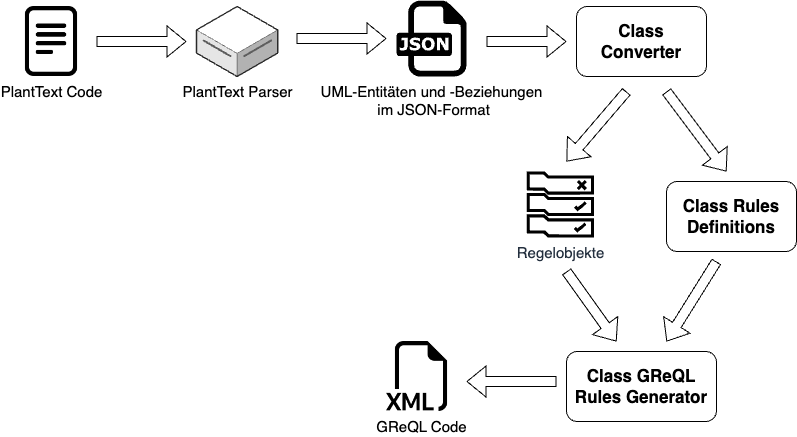
\includegraphics[width=12cm]{images/transit}
    \caption{Repräsentatives Schema des Datentransits im GReQL-Converter.}
    \label{fig:transit}
\end{figure}

\subsection{Prozess der Integration neuer Regeln}

In der Sektion Potenzialen für Weiterentwicklungen genannten Methoden wurde die Möglichkeit diskutiert, neue Regeln
hinzuzufügen. In diesem Abschnitt wird gezeigt, wie dies im Code des GReQL Converters möglich ist. Bei der Entwicklung
wurde stets berücksichtigt, dass das Tool weiter verbessert werden muss. Dies beeinflusste den Entwicklungsprozess,
der darauf abzielte, Abstraktionen zu priorisieren, um eine solide Grundlage für die Verbesserung der
Tool-Funktionalitäten zu schaffen.

Ein Entwickler möchte eine Regel hinzufügen, die die Anzahl der Methoden in einer Klasse bestimmt: ``count\_class\_methods''.
Zunächst muss er die Parameter bestimmen, die diese Regel ausmachen, und sie in der Class Rules Definition definieren.
Im Fall von ``count\_class\_methods'' muss er als Attribut den Klassennamen, der untersucht werden soll, sowie die
Anzahl der Methoden haben. Nach dieser Definition muss der Entwickler eine neue PlantText-Annotation erstellen, um die
Identifizierung dieses neuen Regeltyps durch den ``Class Converter'' zu ermöglichen (unter der Annahme, dass die Regel
aus dem PlantText-Code generiert werden soll und nicht manuell). Nachdem er die Annotation entwickelt hat, muss er
eine Zuordnung zwischen der identifizierten Annotation und der neuen Methode hinzufügen, die er für die Generierung des
JSONs erstellt hat (wie zu Beginn definiert). Um diese Regel für den Lehrer sichtbar und bearbeitbar zu machen, muss er
eine Vue.js-Klasse erstellen, die die grafische Darstellung der Regel darstellt. Abschließend muss er zum ``Class GReQL
Rule Generator'' gehen, um eine neue Regel und eine neue Methode zur Generierung des entsprechenden GReQL-Codes für die
von ihm erstellte neue Regel hinzuzufügen.

Dieser Prozess zur Hinzufügung einer Regel ist für alle Regeln allgemeingültig. Sobald ein Entwickler dies für eine
Regel durchgeführt hat, wird es für andere Entwickler offensichtlich. Der Arbeitsablauf bleibt für fast alle Regeln auf
der Plattform weitgehend gleich.


\subsection{Prozess zur Erweiterung der Kompatibilität mit einer neuen Plattform}


In der Sektion zur Erweiterung der Kompatibilität des GReQL Converters wurde die Möglichkeit diskutiert, die
Unterstützung neuer Plattformen hinzuzufügen. Aktuell ist BOUML die einzige Plattform, die mit dem GReQL Converter
kompatibel ist. Die Hinzufügung der Unterstützung einer neuen Plattform ist jedoch eine Aufgabe, die im GReQL Converter
leicht realisierbar ist. Da sich der Regeltyp und die Parameter nicht ändern, sind keine wesentlichen Änderungen im Code
erforderlich. Der Entwickler muss lediglich eine neue Query zur Vorlage jeder Regel hinzufügen (siehe Code~\ref{lst:example_more_Queries}).
Wenn der GReQL Engine eine Regel auswertet, prüft er lediglich, ob eine der Queries gültig ist. Wenn die Unterstützung
einer neuen Plattform hinzugefügt werden soll, muss der Entwickler nur die Queries der bereits vorhandenen Regeln
vervollständigen, die eine Erweiterung erfordern. Durch diese Methode muss der Entwickler nur an einer einzigen Stelle
im Code Änderungen vornehmen. Der Lehrer muss keine Zielplattform auswählen. Sobald die Unterstützung hinzugefügt und
getestet wurde, kann der Lehrer automatisch GReQL-Code für diese neue Plattform generieren.

\begin{lstlisting}[caption={ Codebeispiel mit mehreren Queries}, label={lst:example_more_Queries}, float=!ht, language=xml]
<rule type="${rule.existence}" points="${rule.points}">
  <!-- Aggregation Regel -->
  <query>
    <!-- Query for BOUML -->
	from x, y : V{Class}, p: V{Property},
        a,b: V{LiteralString} with
	${checkName}
	isDefined(p.aggregation) and
	p.aggregation="composite" and
	x --&gt; V{Property} --&gt; V{Association}
	--&gt; p &lt;-- y and
	report 1 end
  </query>
  <query>
    <!-- Enterprise Architect Query hier schreiben -->
  </query>
  <feedback>${rule.feedback}</feedback>
</rule>
\end{lstlisting}

\subsection{Prozess der Erweiterung um einen neuen Diagrammtypen}


Der GReQL Converter arbeitet nur mit Klassendiagrammen. Es ist jedoch geplant, dass das Tool sich weiterentwickeln kann,
indem es andere Arten von Diagrammen integriert. Um die Unterstützung eines neuen Diagrammtyps hinzuzufügen, muss der
Entwickler zunächst eine Datei ähnlich dem ``Class Converter'' erstellen. Für Sequenzdiagramme könnte dies beispielsweise
``Sequenz Converter'' genannt werden. Es sollte die gleichen Funktionen wie der Class Converter haben, jedoch für
Sequenzdiagramme. Es wird eine Anfrage an den PlantUML-Parser gesendet, der ein Objekt zurückgibt, das die Entitäten
und Beziehungen zwischen den Elementen des Sequenzdiagramms darstellt, das mit PlantText generiert wurde. Anschließend
verwendet der Sequenz Converter eine ``Sequenz Rules Definition''-Datei, um Regeln zu generieren, die auf dem gleichen
Prinzip basieren, das im Abschnitt zum Datentransit im GReQL-Converter beschrieben ist
(siehe Abschnitt~\ref{subsec:datentransit-im-greql-converter}). Danach muss der Entwickler Vue.js-Klassen erstellen, die
zur grafischen Modifikation und Visualisierung jeder dieser Regeln dienen. Abschließend muss der Entwickler einen
``Sequenz GReQL Rules Generator'' erstellen, der den GReQL-Code für jede Regel generiert (basierend auf dem gleichen
Prinzip wie der Class GReQL Rules Generator).

Es ist wichtig zu betonen, dass zusätzliche Änderungen an der Startseite und der Tool-Dokumentation erforderlich sind,
um dem Toolbenutzer zu ermöglichen zu sehen, dass diese Funktionalität bereits möglich ist. Dieser Prozess zur
Hinzufügung eines neuen Diagrammtyps ist generisch. Sobald der Entwickler den Prozess für Klassen verstanden hat, ist es
recht einfach, dasselbe für andere Arten von Diagrammen zu tun. Diese Strategie wurde von Anfang an während der
Entwicklung des Tools konzipiert, um zukünftige Integrationen zu erleichtern.


\section{Zusammenfassung der Diskussion}

Die Entwicklung des GReQL Converters basierte auf der grundlegenden Überlegung, ein Tool zu schaffen, das sich
kontinuierlich weiterentwickeln kann. Dieser Aspekt fand sich in der Gestaltung des Codes wider, der gemäß etablierter
Designprinzipien und bewährter Praktiken verfasst wurde. Der Fokus lag darauf, kommenden Entwicklern, die an diesem Tool
arbeiten, eine klare Orientierung zu bieten und ihre Entwicklererfahrung erheblich zu verbessern, wie auch McConnell es
erwähnt~\cite{mcconnell2006software}. Diese strategische Herangehensweise zielt darauf ab, eine solide Grundlage zu
schaffen, die zukünftige Erweiterungen und Anpassungen erleichtert und einen nahtlosen Entwicklungsprozess für kommende
Versionen des GReQL Converters ermöglicht.
